\documentclass[10pt,a4paper,openany,twoside, eleve]{book}

\usepackage{layout_cours}
\usepackage[hidelinks]{hyperref}

\setlist{leftmargin=5mm}

\begin{document}
\chapnumber{5} % numéro du chapitre
\titre{Dérivation} % titre du chapitre
\classe{Terminale STMG} % classe
\entetegal
\makeatletter
\addcontentsline{toc}{chapter}{Chapitre \@chapnumber - \@titre} % Prepare a table of contents
\makeatother

% Debut du texte  
% **************
\section{Rappels: tangentes, droites et courbes}

\setcounter{sectionexo}{1}

\begin{exon}
  \begin{minipage}[t]{.5\textwidth}
    \vspace{-1.5cm}
    On considère le graphe $\mathcal{C}$ ci-contre.
    \\
    Tracer les tangentes à $\mathcal{C}$ aux points d'abscisse $-0.5$,
    $0$ et $0.5$.
  \end{minipage}%
  \hfill
  \begin{minipage}{.5\textwidth}
    \vspace{-2cm}
    \begin{center}
      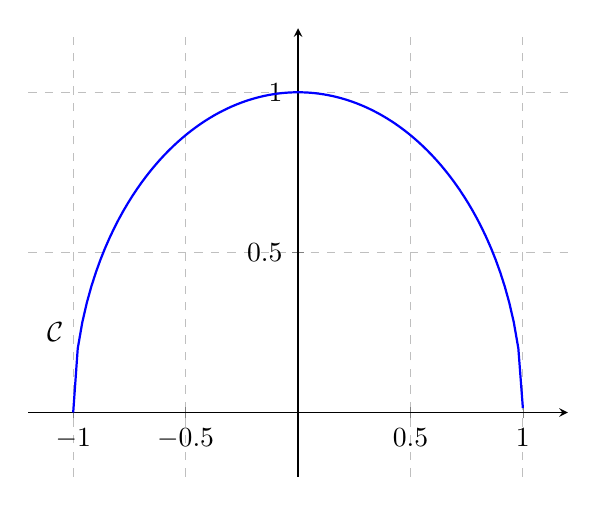
\begin{tikzpicture}
        \begin{axis}[
            axis lines=middle,
            xmin=-1.2, xmax=1.2,
            ymin=-0.2, ymax=1.2,
            xtick={-1,-0.5,0,0.5,1},
            ytick={0,0.5,1},
            samples=100,
            domain=-1:1,
            grid=both,
            grid style=dashed,
          ]
          \addplot[thick,blue] {sqrt(1-x^2)};
          \node[left] at (axis cs:-1,0.25) {$\mathcal{C}$};
        \end{axis}
      \end{tikzpicture}
    \end{center}
  \end{minipage}
\end{exon}

\vspace{5mm}

\begin{exon}
  \begin{minipage}[t]{.5\textwidth}
    \vspace{-8cm}
    La courbe $\mathcal{C}_f$, représentative d'une fonction $f$, est donnée
    ci-dessous.

    \medskip
    Construire les tangentes à cette courbe aux points d'abscisses
    $-5$; $-4$; $-1$; $0$; $2$, $4$ et $5$.
  \end{minipage}
  \hfill
  \begin{minipage}[t]{.5\textwidth}
    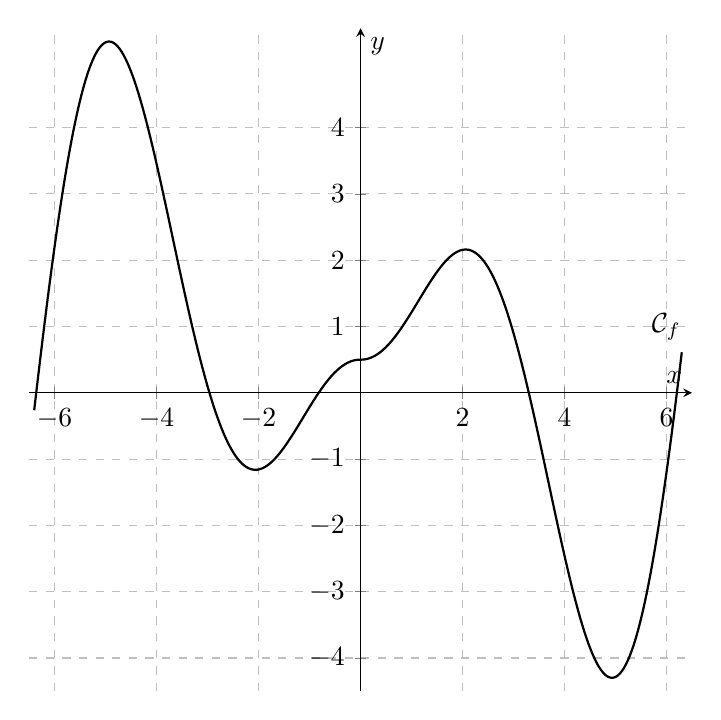
\begin{tikzpicture}
      \begin{axis}[
          axis lines=middle,
          xtick={-6.0,-4.0,...,6.0},
          ytick={-4.0,...,4.0},
          grid=both,
          grid style=dashed,
          xlabel={$x$},
          ylabel={$y$},
          width=10cm,
          height=10cm,
          xmin=-6.5, xmax=6.5,
          ymin=-4.5, ymax=5.5
        ]

        % Plot the function
        \addplot[
          thick,
          samples=500,
          domain=-6.4:6.3,
        ]
        {sin(deg(x))*abs(x)^1.1*0.85+0.5};

        % Label for the curve
        \node at (axis cs:6,1) {$\mathcal{C}_f$};
      \end{axis}
    \end{tikzpicture}
  \end{minipage}
\end{exon}

\begin{exon}
  Un apiculteur produit du miel.
  Le co\^ut de production hebdomadaire de $x$ kilogramme de miel
  est donné, en euros, par l'expression
  $C(x)=0,04x^2+x+150$.

  \begin{minipage}[t]{0.5\textwidth}
    \vspace{-5.5cm}
    \begin{enumerate}
      \item Quel est le montant des co\^uts fixes ?
      \item Calculer le co\^ut de production pour 40 kg de miel,
            puis celui pour 60 kg.
      \item Calculer $C(61)-C(60)$. Que représente cette valeur ?
      \item La courbe représentative de la fonction $C$ est donnée ci-contre.

            Retrouver les co\^uts précédents par lecture graphique.
      \item On note $A$ le point de la courbe d'abscisse $61$
            et $B$ celui d'abscisse $60$.

            Placer les points $A$, $B$ et la droite $(AB)$.

            Tracer la tangente à la courbe au point $A$.
            Que remarque-t'on ?
    \end{enumerate}
  \end{minipage}
  \begin{minipage}[t]{0.5\textwidth}
    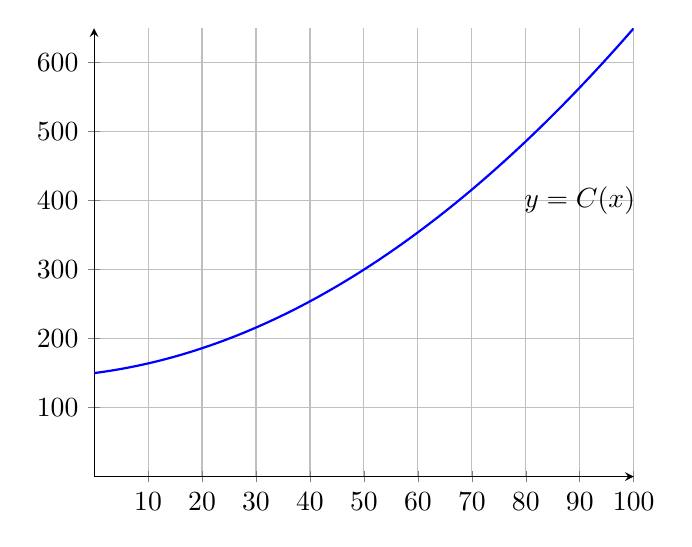
\begin{tikzpicture}
      \begin{axis}[
          axis lines=middle,
          xmin=0, xmax=100,
          ymin=0, ymax=650,
          xtick={10,20,30,40,50,60,70,80,90,100},
          ytick={100,200,300,400,500,600},
          grid=both,
          samples=100,
          domain=0:100
        ]
        \addplot[thick,blue] {0.04*x^2 + x + 150};
        \node at (axis cs:90,400) {$y = C(x)$};
      \end{axis}
    \end{tikzpicture}
  \end{minipage}

\end{exon}

\newpage

\begin{defi}{Tangente à une courbe}{}
  La \textbf{tangente} à une courbe au point $A$ est une droite qui « touche » la courbe au plus près du voisinage du point $A$.
\end{defi}

\begin{defi}{Taux d'accroissement}{}
  On définit un taux d'accroissement $\tau$ par la formule suivante :

  \begin{minipage}[t]{.5\textwidth}
    \vspace{-4.5cm}
    \begin{align*}
      \tau
       & =\frac{\text{variation d'ordonnées }\Delta y}{\text{variation d'abscisses }\Delta x} \\
       & =\frac{y_A-y_B}{x_A-x_B}
    \end{align*}
  \end{minipage}
  \hfill
  \begin{minipage}[t]{.5\textwidth}
    \begin{center}
      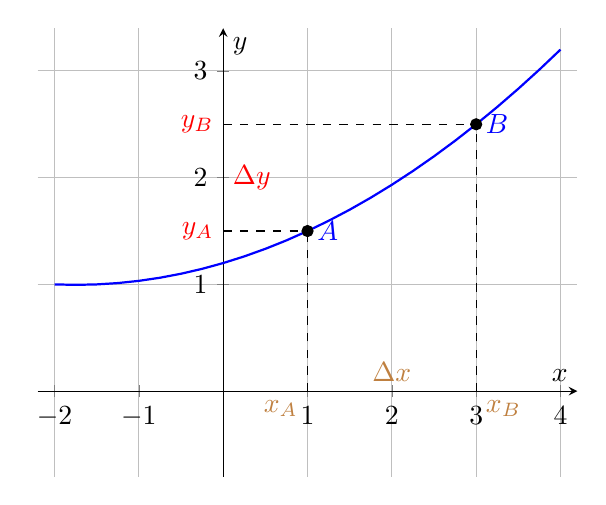
\begin{tikzpicture}
        \begin{axis}[
            axis lines=middle,
            xmin=-2.2, xmax=4.2,
            ymin=-0.8, ymax=3.4,
            xlabel={$x$},
            ylabel={$y$},
            grid=major,
            xtick={-2,-1,0,1,2,3,4},
            ytick={-2,-1,0,1,2,3,4}
          ]
          % Définition des points
          \addplot[blue, domain=-2:4, thick] {0.4*(x-1)*(x-3)-0.75*x*(x-3)+2.5/6*x*(x-1)};
          \addplot[only marks, mark=*] coordinates {(1,1.5) (3,2.5)};

          % Pointillés pour montrer les variations
          \draw[dashed] (axis cs:1,0) node[below left, brown] {$x_A$} -- (axis cs:1,1.5) node[right, blue] {$A$};
          \draw[dashed] (axis cs:3,0) node[below right, brown] {$x_B$}-- (axis cs:3,2.5) node[right, blue] {$B$};
          \draw[dashed] (axis cs:0,1.5) node[left, red] {$y_A$} -- (axis cs:1,1.5);
          \draw[dashed] (axis cs:0,2.5) node[left, red] {$y_B$} -- (axis cs:3,2.5);

          % Labels pour les variations
          \node[above, brown] at (axis cs:2,0) {$\Delta x$};
          \node[right, red] at (axis cs:0,2) {$\Delta y$};
        \end{axis}
      \end{tikzpicture}
    \end{center}
  \end{minipage}
\end{defi}

\begin{ex}{}{}
  Dans l'exemple ci-dessus, le taux d'acroissement $\tau$ vaut :
  \begin{reponse}
    \begin{align*}
      \tau
       & =\frac{\text{variation d'ordonnées }\Delta y}{\text{variation d'abscisses }\Delta x} \\
       & =\frac{2.5-1.5}{3-1}                                                                 \\
       & =\frac{1}{2} = 0.5
    \end{align*}
  \end{reponse}
\end{ex}


\begin{exon}
  Soit $\fonction{r}{\fo{0}{+\infty}}{\R}{x}{f(x)}$ la fonction qui donne la rentabilité du producteur en fonction du nombre $x$ d'unités produites.

  \begin{minipage}[t]{.5\textwidth}
    \vspace{-4.5cm}
    \begin{enumerate}
      \item A l'aide de la courbe calculer le taux d'accroissement $\tau$ de $r$ entre $x_1=10$ et $x_2=30$.
      \item De quel signe est le taux d'accroissement ? Comment interpréter cette donnée ?
      \item A l'aide de la courbe calculer le taux d'accroissement $\tau$ de $r$ entre $x_2=30$ et $x_3=50$ ?
      \item De quel signe est le taux d'accroissement ? Comment interpréter cette donnée.
      \item Quel est le nombre $x$ d'unités à produire qui garantit un bénéfice maximal ?
    \end{enumerate}
  \end{minipage}
  \hfill
  \begin{minipage}[t]{.5\textwidth}
    \begin{center}

      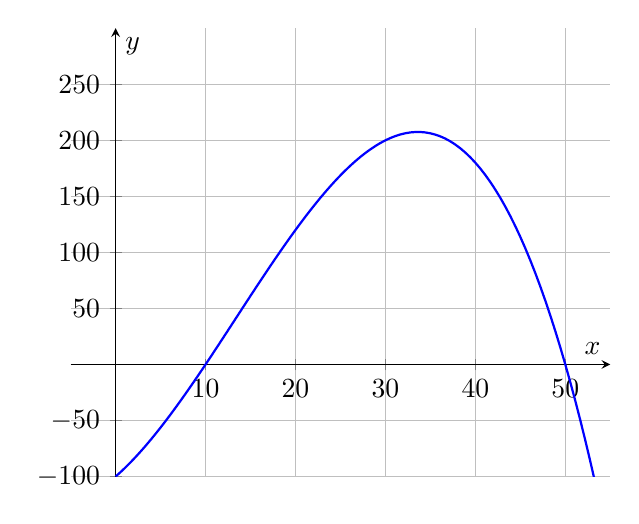
\begin{tikzpicture}
        \begin{axis}[
            axis lines=middle,
            xtick={0,10, ...,50},
            ytick={-100, -50,...,250},
            grid=both,
            samples=100,
            xlabel={$x$},
            ylabel={$y$},
            xmin=-5, xmax=55,
            ymin=-100, ymax=300,
          ]

          \addplot[blue, domain=0:55, thick] {(x-10)*(x-30)*(x-50)/150-x*(x-10)*(x-50)/60};
        \end{axis}
      \end{tikzpicture}
    \end{center}
  \end{minipage}

  \vspace{4mm}

  \dotsfill{9}
\end{exon}

\newpage

\begin{defi}{Coefficient directeur d'une droite}{}
  Le \textbf{coefficient directeur} d'une droite d'équation $y=mx+b$ est le nombre $m$ qui détermine sa pente.
\end{defi}

\begin{prop}{Sens de croissance d'une fonction affine}{}
  Soit $m \ne 0$ et $b\in\R$. Soit $\fonction{f}{\R}{\R}{x}{mx+b}$ une fonction affine. Sa courbe representative est la droite d'équation $y=mx+b$.

  \begin{itemize}
    \item Si $m>0$, alors la fonction $f$ est croissante et la droite "monte".
    \item Si $m<0$, alors la fonction $f$ est décroissante et la droite "descend".
  \end{itemize}
\end{prop}

\begin{prop}{Taux d'accroissement d'une fonction affine}{}
  Le taux d'accroissement $\tau$ d'une fonction affine est constant et vaut la pente $m$ de la droite.

  \begin{minipage}[t]{.5\textwidth}
    \vspace{-4.5cm}
    \begin{align*}
      \tau & = m                                                                                  \\
           & =\frac{\text{variation d'ordonnées }\Delta y}{\text{variation d'abscisses }\Delta x} \\
           & =\frac{y_A-y_B}{x_A-x_B}
    \end{align*}
  \end{minipage}
  \hfill
  \begin{minipage}[t]{.5\textwidth}
    \begin{center}
      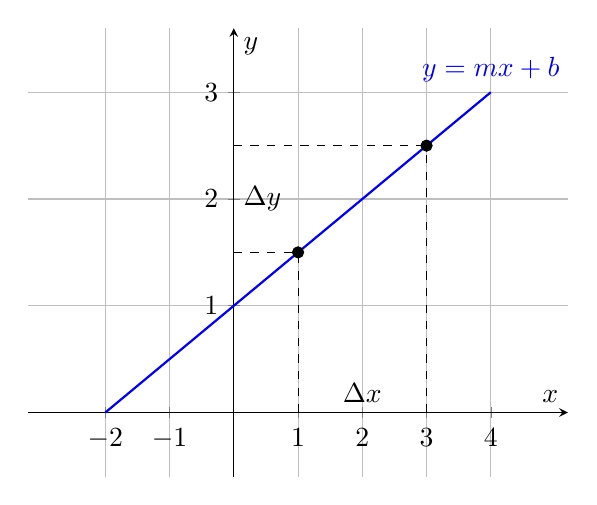
\begin{tikzpicture}
        \begin{axis}[
            axis lines=middle,
            enlargelimits=0.2,
            xlabel={$x$},
            ylabel={$y$},
            grid=major,
            xtick={-2,-1,0,1,2,3,4},
            ytick={-2,-1,0,1,2,3,4}
          ]
          % Définition des points
          \addplot[blue, domain=-2:4, thick] {0.5*x + 1} node[above] {$y = mx + b$};
          \addplot[only marks, mark=*] coordinates {(1,1.5) (3,2.5)};

          % Pointillés pour montrer les variations
          \draw[dashed] (axis cs:1,0) -- (axis cs:1,1.5);
          \draw[dashed] (axis cs:3,0) -- (axis cs:3,2.5);
          \draw[dashed] (axis cs:0,1.5) -- (axis cs:1,1.5);
          \draw[dashed] (axis cs:0,2.5) -- (axis cs:3,2.5);

          % Labels pour les variations
          \node[above] at (axis cs:2,0) {$\Delta x$};
          \node[right] at (axis cs:0,2) {$\Delta y$};
        \end{axis}
      \end{tikzpicture}
    \end{center}
  \end{minipage}

\end{prop}


\begin{exon}
  \begin{minipage}[t]{.5\textwidth}
    \vspace{-5cm}
    \begin{enumerate}
      \item Tracer dans un repère les droites

            $D_1$ d'équation $y=0.5x-1$

            $D_2$ d'équation $y=-x+2$.
      \item Quel est le coefficient directeur de la droite $D_1$? Et pour la droite $D_2$?
      \item Soit $\fonction{f_1}{\R}{\R}{x}{0.5x-1}$.

            Que vaut le taux d'accroissement $\tau$ de $f$ entre $x_1=1$ et $x_2=3$ ?
    \end{enumerate}
  \end{minipage}
  \hfill
  \begin{minipage}[t]{.5\textwidth}
    \begin{center}
      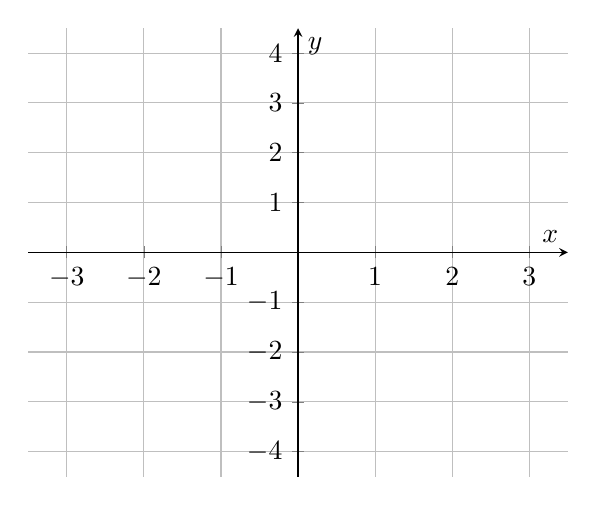
\begin{tikzpicture}
        \begin{axis}[
            axis lines=middle,
            xtick={-3,...,3},
            ytick={-4,...,4},
            grid=both,
            samples=100,
            xlabel={$x$},
            ylabel={$y$},
            xmin=-3.5, xmax=3.5,
            ymin=-4.5, ymax=4.5,
          ]
        \end{axis}
      \end{tikzpicture}
    \end{center}
  \end{minipage}

  \vspace{5mm}

  \dotsfill{18}
\end{exon}

\newpage

% \begin{exon}
%   Chaque jour, une entreprise fabrique $x$ centaines de cartons d'emballage,
%   $x$ compris entre 0 et 12.
%   \\
%   Le co\^ut total de la fabrication journalière de ces cartons, en euros,
%   est exprimé par
%   $f(x)=x^3-12x^2+50x+126$.

%   La recette journalière totale, en euros, pour $x$ centaines de cartons vendues
%   est donnée par la fonction $r$.

%   On donne ci-après un tracé des courbes représentatives de $f$ et $r$.

%   \begin{tikzpicture}
%     \begin{axis}[
%         width=12cm, height=10cm,
%         axis lines=middle,
%         xmin=0, xmax=13,
%         ymin=-30, ymax=850,
%         xtick={1,2,3,4,5,6,7,8,9,10,11,12},
%         ytick={100,200,300,400,500,600,700,800},
%         grid=major,
%         xlabel={$x$},
%         ylabel={$y$},
%         legend pos=north west
%       ]
%       % Plot f(x) = x^3 - 12x^2 + 50x + 126
%       \addplot[domain=0:12, thick, blue, samples=100] {x^3 - 12*x^2 + 50*x + 126};
%       \addlegendentry{$f$}

%       % Plot r(x) = 50x
%       \addplot[domain=0:12, thick, red, samples=100] {50*x};
%       \addlegendentry{$r$}
%     \end{axis}
%   \end{tikzpicture}

%   \begin{enumerate}
%     \item Déterminer le montant des charges fixes.
%     \item Quel est le prix de vente de 100 cartons ?
%     \item Exprimer $r(x)$ en fonction de $x$.
%     \item \'Etablir à partir du graphique le tableau de variation
%           de la fonction $f$.
%     \item Déterminer graphiquement l'intervalle auquel doit appartenir le
%           nombre de cartons que l'entreprise doit fabriquer et vendre
%           pour réaliser un bénéfice.
%     \item On suppose que tout carton fabriqué est vendu, et on note $b(x)$
%           le bénéfice journalier.

%           \begin{enumerate}[label=\alph*]
%             \item Exprimer $b(x)$ en fonction de $x$.
%             \item Tracer la courbe du bénéfice $b$, par exemple à l'aide de la
%                   calculatrice, et dresser son tableau de variation.
%             \item En déduire le nombre de cartons à fabriquer chaque jour pour
%                   réaliser le bénéfice maximal.
%           \end{enumerate}
%   \end{enumerate}
% \end{exon}

\newpage
\section{Calcul de la fonction dérivée}

\begin{defi}{Nombre dérivée}{}
  La fonction $f$ est \textbf{dérivable} si la taux d'acroissement
  \begin{align*}
    \tau = \frac{f(x+h)-f(x)}{h}
  \end{align*}
  Admet une limite finie lorsque $h\rightarrow 0$. Cette limite est le \textbf{nombre dérivée} en $x$ et on le note $f'(x)$.
\end{defi}

\begin{rem}{}{}
  Lorsqu'on regarde le taux d'acroissement entre deux points éloignés (par exemple, entre $x_A=1$ et $x_B=5$), alors la droite définie par les points $(x_A;y_A)$ et $(x_B;y_B)$ est différente de la tangente.

  En revanche, lorsque $x_A$ et $x_B$ sont proches, alors \textbf{cette droite et la tangente se rapprochent}.

  On peut le visualiser sur \href{https://www.geogebra.org/m/an6GkSqT}{géogebra}.
\end{rem}

\begin{prop}{Règle de calcul d'une fonction dérivée}{}
  On calcule la fonction dérivée d'une fonction quelconque à partir
  des deux tableaux suivants:


  \begin{minipage}[t]{.5\textwidth}
    \centerline{\bf{Dérivées des fonctions usuelles}}

    \[\begin{tabular}{|l|c|}\hline
        \raisebox{0.4cm}[1.2cm]{Fonction $f$}         &
        \raisebox{0.4cm}[1.2cm]{Dérivée}
        \\\hline
        \raisebox{0.1cm}[0.6cm]{$f(x)=k$ (constante)} &
        \raisebox{0.1cm}[0.6cm]{$f'(x)=0$}
        \\\hline
        \raisebox{0.1cm}[0.6cm]{$f(x)=x$}             &
        \raisebox{0.1cm}[0.6cm]{$f'(x)=1$}
        \\\hline
        \raisebox{0.3cm}[1.1cm]{$f(x)=x^2$}           &
        \raisebox{0.3cm}[1.1cm]{$f'(x)=2x$}
        \\\hline
        \raisebox{0.3cm}[1.1cm]{$f(x)=x^3$}           &
        \raisebox{0.3cm}[1.1cm]{$f'(x)=3x^2$}
        \\\hline
      \end{tabular}\]
  \end{minipage}
  \begin{minipage}[t]{.5\textwidth}
    \centerline{\bf{Opérations sur les dérivées}}

    \[\begin{tabular}{|c|c|}\hline
        \raisebox{0.4cm}[1.2cm]{Fonction}                     &
        \raisebox{0.4cm}[1.2cm]{Dérivée}
        \\\hline
        \raisebox{0.1cm}[0.7cm]{$ku$, $(k \text{constante})$} &
        \raisebox{0.1cm}[0.7cm]{$ku'$}
        \\\hline
        \raisebox{0.1cm}[0.7cm]{$u+v$}                        &
        \raisebox{0.1cm}[0.7cm]{$u'+v'$}
        \\\hline
      \end{tabular}\]
  \end{minipage}
\end{prop}



\begin{exon}
  Déterminer la fonction dérivée $f'$ de la fonction $f$ dans chacun des
  cas:

  \begin{tabular}{llll}
    a) $f(x)=3$
     & b) $f(x)=x^2$
     & c) $f(x)=x^7$
     & d) $f(x)=4x^2$
    \\[0.4cm]
    e) $f(x)=5x^3$
     & f) $f(x)=-3x^2$
     & g) $f(x)=7x$
     & h) $f(x)=2x^3+x$
    \\[0.4cm]
    i) $f(x)=-4x^3+2x+3$
     & j) $f(x)=-x+3$
     & k) $f(x)=(3x+2)x^2$
     & l) $f(x)=(-2x+1)(x+1)$
    \\[0.4cm]
    m) $f(x)=\dfrac{x+2}{3x}$
     & n) $f(x)=-x^3+4x$
     & o) $f(x)=\dfrac{-x^3+4x}{x}$
    \\[0.4cm]
  \end{tabular}

  \vspace{5mm}
  \dotsfill{18}
\end{exon}

\begin{exon}
  Une entreprise fabrique chaque semaine $x$ hectolitres d'un certain produit.
  Le co\^ut de fabrication, en euros, de ces $x$ hectolitres de produit est donné
  par
  $C(x)=x^3-90x^2+2700x$, pour $x\geqslant0$.

  On suppose que toute la production est vendue
  au prix de 900 euros l'hectolitre.

  La recette hebdomadaire est alors, en euros,
  donnée par $R(x)=900x$.

  \begin{enumerate}
    \item Exprimer en fonction de $x$ le bénéfice hebdomadaire $B(x)$.
    \item
          \begin{enumerate}[label=\alph*]
            \item On appelle co\^ut marginal du x-ième hectolitre
                  le co\^ut de ce x-ième hectolitre, seul, produit.

                  Quel est le co\^ut marginal du 10ème hectolitre ? du 20ème ?


            \item
                  On utilise généralement l'expression de la dérivée $C'(x)$
                  pour exprimer le co\^ut marginal.

                  Donner l'expression de $C'(x)$,
                  puis calculer $C'(10)$ et $C'(20)$.
                  Comparer avec les cou\^uts marginaux calculés précédemment.

            \item De m\^eme, la recette marginale du x-ième hectolitre
                  est la recette apportée par le x-ième hectolitre, seul.

                  On utilise là aussi généralement l'expression de la dérivée $R'(x)$
                  pour exprimer la recette marginale.

                  Donner l'expression de $R'(x)$ puis calculer les recettes marginales
                  pour 10 hectolitres, puis 20 hectolitres.
          \end{enumerate}

    \item On admet qu'il est renatble pour une entreprise d'augmenter
          sa production tant que $C'(x)<R'(x)$ et $B(x)>0$.

          Analyser la rentabilité d'une augmentation de la production de l'entreprise
          pour les valeurs $x$ suivantes:
          $x=20$; $x=35$, $x=40$; $x=55$; $x=70$.
  \end{enumerate}

  \vspace{5mm}
  \noindent\dotsfill{30}
\end{exon}

\newpage

\section{Sens de variation}

Le sens de variation d'une fonction est donné par le signe de sa dérivée:
\begin{prop}{Nombre dérivée et sens de variation}{}
  Si, sur un intervalle $I$,
  \begin{itemize}
    \item $f'(x)\geqslant0$, alors $f$ est croissante
    \item $f'(x)\leqslant0$, alors $f$ est décroissante
  \end{itemize}
\end{prop}

\begin{dem}{}{}
  \dotsfill{5}
\end{dem}

\begin{exon}
  Soit $f$ la fonction définie sur $[-0,5;9]$
  par $f(x)= -3x^2+7$.
  \begin{enumerate}
    \item Calculer la dérivée de $f$.
    \item Etudier le sens de variation de $f$.
    \item Préciser ses éventuels extremums.
    \item Représente la courbe de la fonction avec ta calculatrice et vérifie tes réponses.
  \end{enumerate}
    
  \vspace{4mm}
  \noindent\dotsfill{12}
\end{exon}

\begin{exon}
  \'Etudier le sens de variation de la fonction $f$ définie
  sur $[-6;5]$ par
  $f(x)=2x^3-3x^2-12x+1$.
    
  \vspace{4mm}
  \noindent\dotsfill{8}
\end{exon}

\newpage
\begin{exon}
 \textbf{Durée du jour et Ramadan}
  
 Certains élèves de STMG font le Ramadan et ne peuvent manger que lorsque la nuit est tombée. La durée d'une journée varie au cours de l'année. La courbe donnant la durée d'une journée est donnée ci-dessous.

 \begin{minipage}{.5\textwidth}
 \begin{center}
  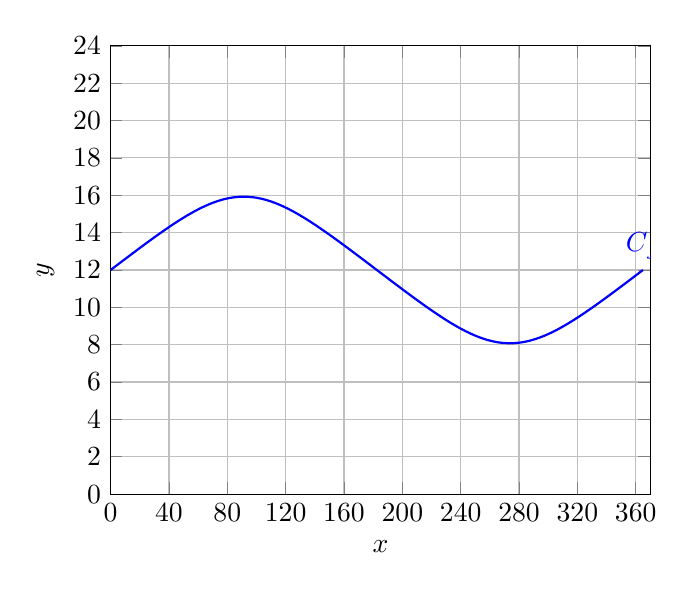
\begin{tikzpicture}
    \begin{axis}[
        xtick={0, 40, ..., 365},
        ytick={0,2, ..., 24},
        xmin=0, xmax=370,
        ymin=0, ymax=24,
        grid=both,
        samples=100,
        xlabel={$x$},
        ylabel={$y$},
      ]
      \addplot[blue, domain=0:365, thick] {-2/15*acos(tan(48.5)*tan(asin(sin(23.5)*sin(x*72/73))))+24} node[above] {$\mathscr{C}_f$};
    \end{axis}
  \end{tikzpicture}
\end{center}
\end{minipage}
\begin{minipage}{.5\textwidth}
\begin{center}
  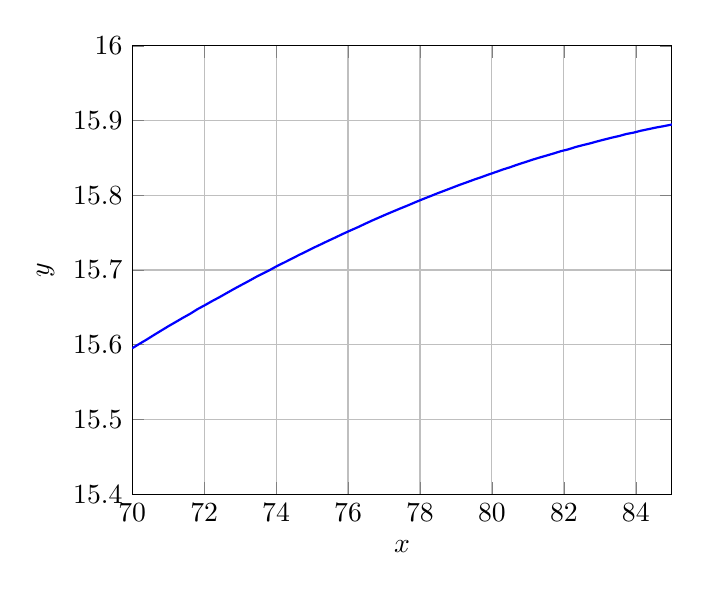
\begin{tikzpicture}
    \begin{axis}[
        xtick={70, 72, ..., 84},
        ytick={15.4, 15.5,...,16},
        xmin=70, xmax=85,
        ymin=15.4, ymax=16,
        grid=both,
        samples=100,
        xlabel={$x$},
        ylabel={$y$},
      ]
      \addplot[blue, domain=70:90, thick] {-2/15*acos(tan(48.5)*tan(asin(sin(23.5)*sin(x*72/73))))+24} node[above] {$\mathscr{C}_f$};
    \end{axis}
  \end{tikzpicture}
  \textbf{
    Zoom sur les jours $\ff{70}{85}$.
  }
\end{center}
\end{minipage}

\begin{enumerate}
  \item Quel est le nombre $a$ de jours qui se sont écoulés depuis le début de l'année ?
  \item Calculer le taux d'acroissement $\tau$ entre aujourd'hui et demain.
  \item De quel signe est le taux d'acroissement ? Quelle est la conséquence sur l'heure de levée du Soleil demain par rapport à aujourd'hui ?
  \item Donne une approximation du nombre dérivée $f'(a)$ à la date d'aujourd'hui.
\end{enumerate}

\vspace{4mm}
\noindent\dotsfill{10}

\end{exon}
% \begin{exon}
%   \'Etudier le sens de variation de chacune des fonctions suivantes:
%   \begin{enumerate}[label=\alph*]
%     \item $f(x)=-3x^3+2$ sur $[-2;3]$
%     \item $f(x)=-x^3+2,25x^2+3x+1$ sur $[-1;3]$
%     \item $f(x)=\dfrac{2}{1+x^2}$ sur $[-1;2]$
%     \item $f(x)=\dfrac{-2x+3}{x-2}$ sur $]2;+\infty[$
%     \item $f(x)=4x-\dfrac{16}{x}$ sur $[0,5;10]$
%     \item $f(x)=x+2+\dfrac{4}{x}$ sur $]0;+\infty[$
%     \item$f(x)=\dfrac{x^2+9}{x}$ sur $[1;4]$
%   \end{enumerate}
% \end{exon}

\section{Equation de la tangente}

\begin{prop}{Equation de tangente et nombre dérivé}{}
  Soit une fonction $f$ dérivable sur $\R$. La droite tangente à la courbe au point d'abscisse $a\in\R$ a pour équation :
  \begin{align*}
    y = f'(a)(x-a) + f(a) = f'(a)x + f(a)-a*f'(a)
  \end{align*}

  Le coefficient directeur (pente) est $m=f'(a)$. C'est le nombre dérivée à l'abscisse $a$.

  L'ordonnée à l'origine vaut $b=f(a)-a*f'(a)$
\end{prop}

\begin{rem}{}{}
  On peut vérifier que pour $x=a$, la droite « touche » la courbe car $y = f'(x)*0 + f(a) = f(a)$.
\end{rem}

\begin{exon}
  Soit $f(x)=3x^2+5$.
  Déterminer l'équation de la tangente à la courbe de $f$ au point
  d'abscisse~$a=1$.

  \vspace{4mm}
  \dotsfill{3}
\end{exon}

\begin{exon}
  Soit $f(x)\!=\! 4x(2x+1)$.
  Déterminer l'équation de la tangente à la courbe de $f$ au point
  d'abscisse~$a\!=\!1$.

  \vspace{4mm}
  \dotsfill{5}
\end{exon}

\begin{exon}
  Soit $f(x)\!=\!5x+\dfrac{4x^2+7x}{x}$.
  Déterminer l'équation de la tangente à la courbe de $f$ au point
  d'abscisse~$a\!=\!2$.

  \vspace{4mm}
  \dotsfill{5}
\end{exon}


\begin{exon}
  Soit $f(x)\!=\!\dfrac{2x+1}{x+2}$.
  Déterminer l'équation de la tangente à la courbe de $f$ au point
  d'abscisse~$a\!=\!2$.
  
  \vspace{4mm}
  \dotsfill{5}
\end{exon}



\newpage
\section{Exercices}

\begin{exon} \textbf{(BAC)}
  Un artisan fabrique et vend des objets en bois.
  Pour chaque mois, il estime que le co\^ut de production de $x$ objets
  est donné, en euros, par:
  $C(x)=x^2+60x+121$,
  pour $1\leqslant x\leqslant 30$.

  \begin{enumerate}
    \item Calculer le co\^ut de production de 10 objets, puis de 30 objets.

          Donner alors le co\^ut moyen de production de 10 objets, puis de 30 objets.

    \item Plus généralement, le co\^ut moyen de production
          est donné par $f(x)=\dfrac{C(x)}{x}$.

          \begin{enumerate}[label=\alph*]
            \item Montrer que $f(x)=x+60+\dfrac{121}{x}$.
            \item Calculer $f'(x)$ et montrer que $f'(x)=\dfrac{x^2-121}{x^2}$.
                  Dresser alors le tableau de variation de $f$.

            \item Quel est le co\^ut moyen minimum ? pour combien d'objets produits ?
          \end{enumerate}

    \item L'artisan vend chaque objet 110 euros.
          \begin{enumerate}[label=\alph*]
            \item Expliquer pourquoi le bénéfice mensuel réalisé par la fabrication
                  et la vente de $x$ objets est égal~à:
                  $B(x)=-x^2+50x-121$.

            \item Dresser le tableau de signes de $B(x)$.
                  Combien d'objets faut-il fabriquer au minimum pour \^etre rentable ?

            \item Calculer $B'(x)$ et étudier son signe.

                  En déduire le nombre d'objets à fabriquer et à vendre pour que ce bénéfice
                  soit maximal.
                  Donner ce bénéfice maximal.
          \end{enumerate}

  \end{enumerate}
\end{exon}


\begin{exon} \textbf{Vrai-Faux}

  Un tracé de la courbe $\mathcal{C}$ représentative de la fonction $f$
  définie sur l'intervalle $[0;10]$ par
  $f(x)=x^3-48x+600$ est donné ci-dessous.

  La droite $D$ d'équation $y=99x$ est aussi représentée.

  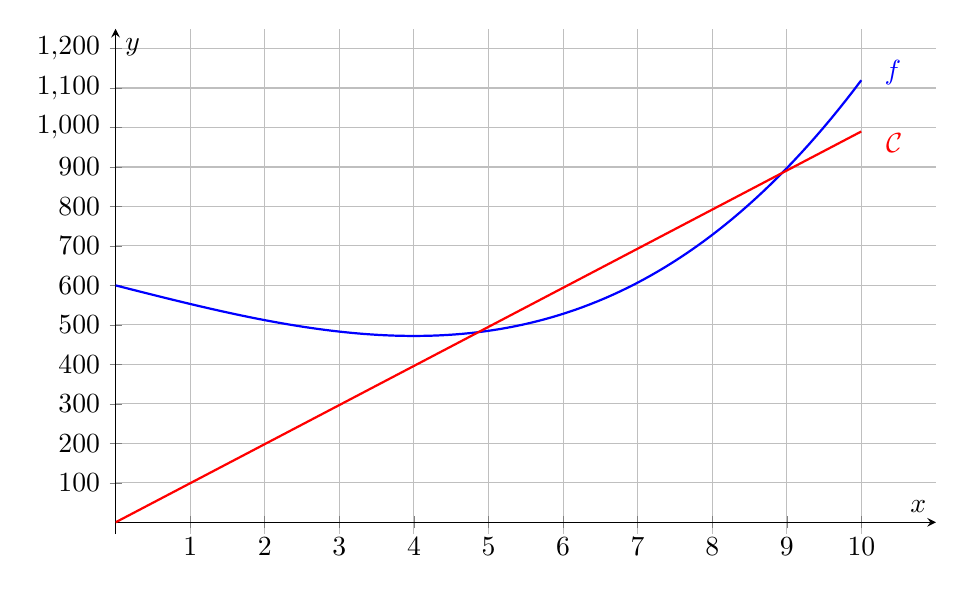
\begin{tikzpicture}
    \begin{axis}[
        width=12cm, height=8cm,
        axis lines=middle,
        xmin=0, xmax=11,
        ymin=-30, ymax=1250,
        xtick={1,2,3,4,5,6,7,8,9,10},
        ytick={100,200,300,400,500,600,700,800,900,1000,1100,1200},
        grid=major,
        xlabel={$x$},
        ylabel={$y$}
      ]

      % Plot f(x) = x^3 - 48x + 600
      \addplot[thick, blue, samples=100, domain=0:10] {x^3 - 48*x + 600};

      % Plot linear function g(x) = 99x
      \addplot[thick, red, samples=100, domain=0:10] {99*x};

      % Labels
      \node[right] at (axis cs:10.2,960) {\color{red} $\mathcal{C}$};
      \node[right] at (axis cs:10.18,1140) {\color{blue} $f$};

    \end{axis}
  \end{tikzpicture}

  Répondre par vrai ou faux en justifiant.

  \begin{enumerate}
    \item On peut conjecturer que $f$ est strictement croissante sur $[0;10]$.
    \item $f(0)=600$
    \item $f(7)=600$
    \item $f'(x)=3(x-4)(x+4)$
    \item Pour tout $x$ de $[4;10]$, $f'(x)\geqslant0$
    \item $f$ a un minimum en $x=4$
    \item Pour tout $x$ de $[0;10]$, $f(x)\geqslant472$
    \item La tangente à $\mathcal{C}$ au point d'abscisse 2
          a un coefficent directeur positif
    \item L'équation réduite de la tangente à $\mathcal{C}$ au point
          d'abscisse 6 est $y=60x+168$
    \item Pour tout $x$ de $[4;9]$, $f(x)\leqslant 99x$.
  \end{enumerate}
\end{exon}


\begin{exon}
  Le ministère de la santé charge une agence de publicité de faire
  une campagne de promotion pour un nouveau remède.
  Une étude prouve que la fréquence $f(t)$ de personnes connaissant
  le nom de ce remède après $t$ semaines de publicité est donnée
  par $f(t)=\dfrac{3t}{3t+2}$, où $t\geqslant0$.

  \textbf{Partie A.}
  \begin{enumerate}
    \item Calculer $f(2)$.
    \item En déduire le pourcentage de personnes qui ignorent le nom
          de ce remède au bout de deux semaines.
    \item Comment peut-on interpréter la valeur de $f(0)$ ?
  \end{enumerate}

  \textbf{Partie B.}
  \begin{enumerate}
    \item Calculer $f'(t)$.

          \'Etudier le sens de variation de la fonction $f$ sur
          l'intervalle $[0;18]$;
    \item
          \begin{enumerate}[label=\alph*]
            \item Tracer l'allure courbe représentative $\mathcal{C}$ de $f$.
            \item Déterminer l'équation réduite de la tangente $T$ à $\mathcal{C}$
                  au point $A$ d'abscisse 1.
            \item Ajouter au graphique précédent la droite $T$.
            \item Ajouter au graphique précédent les droites
                  $D$ d'équation $y=0,90$ et $D'$ d'équation $y=0,95$.
          \end{enumerate}
  \end{enumerate}

  \textbf{Partie C.}
  \begin{enumerate}
    \item Déterminer graphiquement:
          \begin{enumerate}[label=\alph*]
            \item le nombre de semaines de campagne nécessaires pour que 90\%
                  de la population connaisse le nom du remède;
            \item combien de semaines sont nécessaires pour passer de 90\%
                  à 95\%
          \end{enumerate}
    \item le ministère a décidé d'arr\^eter la campagne au bout de six semaines.
          Justifier ce choix.
  \end{enumerate}
\end{exon}

%**************
% Fin du texte

\end{document}

